% Készítette: Hajnal Máté
% Az Elte Programtervező Informatikus szakához tartozó Programozás tantárgyhoz tartozó házi feladatom.
% A feladatok közül a 11-es

\documentclass[12pt,a4paper]{article}			%Article dokumentum
\usepackage[utf8]{inputenc}						%UTF-8-as kódolás
\usepackage{t1enc}								%Furcsa betűk
\usepackage{fancyhdr}							%For footer and header

%LANGUAGE-FONT
%texlive-lang-hungarian package should be installed!
\usepackage[english,magyar]{babel}				%Magyar nyelv 
\usepackage{mathptmx}							%Times New Roman font
\usepackage[shortlabels]{enumitem}							%For enumerations
\usepackage{url}								%For URL-s
\usepackage[headheight=56pt]{geometry}			%For the heading gap

%MATHEMATICAL EXPRESSIONS
\usepackage[fleqn]{amsmath}						%Mathematical expressions
\usepackage{amsfonts}							%Mathematical fonts
\usepackage{bm}									%Bolding

%TABLES, TABULATING, DRAWING
\usepackage{array}
\usepackage{tabu}
\usepackage{multirow}
\usepackage{tabularx}
\usepackage{tikz}
\usepackage{stuki}

%HEADER
\sloppy
\fancyhead{}
\fancyhead[C]{\textbf{1.beadandó feladat/11.feladat}}
\fancyhead[R]{\today}
\fancyhead[L]{Hajnal~Máté \newline RJBSCJ \newline \url{hajnalmt@inf.elte.hu} \newline 5.csoport}
\pagestyle{fancy}

%Fejezet stílus deklaráció
\newcommand{\fejezet}[1]{\noindent \textbf{\textit{\large #1 \vspace{5mm}}}}

%DOCUMENT
\begin{document}
	\pagenumbering{arabic}
	
	%% Feladat fejezet %%
	\fejezet{Feladat}\\
	\textit{Egy határállomáson feljegyezték az átlépő utasok útlevélszámát. Melyik útlevélszámú
	utas fordult meg leghamarabb másodszor a határon?}
	\vspace{5mm}

	%% Specifikáció fejezet %%
	\fejezet{Specifikáció}\\
	Az értékeket egy tömbben tároljuk. 
		% A feladat definiálása, Adathalmaz, Előfeltétel, Utófeltétel %
		\begin{flalign*}
			&A=(t:String^n,~min:\mathbb{N},~ind:\mathbb{N},~l:\mathbb{L})\\
			&Ef=(t=t')\\
			&Uf=(Ef~\wedge~min, ind, l = \min _{i=1,~Vanmasodik() = igaz}^{i=n-1}(Vanmasodik()))\\
			& ahol~Vanmasodik() = search_{k=i+1}^{n} t[i]=t[k]
		\end{flalign*}
	
	%% Algoritmus fejezet %%
	\fejezet{Algoritmus}\\
	A feladatot a feltételes maximumkeresés tételére vezetjük vissza, csak esetünkben minimumkereséssel. Továbbá a második elem megkeresése egy pesszimista lineáris kereséssel $Vanmasodik()$ oldható meg. Érdekes megfigyelés, hogy a lineáris keresés eredményét kapja meg feltételként és bemenetként is a feltételes maximum keresés. A struktogrammok az alábbiak: \vspace{5mm}\\
		% Megfeleltetés%
		\noindent\hfill
		\begin{stukibox}[6cm]
			\stm*{\bfseries{felt. max. ker.}}
			\stm*[4]{i:m..n $\sim$ 1..n-1 \\ $\beta(i) \sim$ Vanmasodik()=igaz \\ f(i) $\sim$ Vanmasodik()}
		\end{stukibox}
		\hfill
		\begin{stukibox}[4cm]
			\stm*{\bfseries{pessz. lin. ker.}}
			\stm*[4]{k:m..n $\sim$ i+1..n \\ $ \beta(i) \sim$ t[i] = t[k] }
		\end{stukibox}
		\hfill{}

		\noindent\hfill
		\begin{stuki}[\textwidth]
			\stm*{l, min, ind:=hamis, n, 0}
			\begin{WHILE}{4}{\stm{i=0..n-1}}
				\stm{j,l_2=Vanmasodik()}
				\begin{CASE}[1]{2}{6}
				\WHEN[1] {\stm[1]{\lnot l_2 }}
					\stm*[1]{SKIP}
				\WHEN[3] {\stm[1]{l_2 \land l}}
					\begin{IF}{1}{\stm{min>j}}
						\stm{min,ind=j,i}
					\ELSE
						\stm*{SKIP}
					\end{IF}
				\WHEN[2] {\stm[1]{l_2 \land \lnot l}}
					\stm[1]{l, min, ind = igaz, j, i}
				\end{CASE}
			\end{WHILE}
		\end{stuki}
		\begin{stuki*}{Vanmasodik} 
			\stm{l_2, j:= hamis, i}
			\begin{WHILE}{2}{\stm{k=i+1..n}}
				\begin{IF}{1}{\stm{t[i]=t[k] \land \lnot l_2}}
					\stm{l_{2}, j := igaz, k}
				\ELSE
					\stm{SKIP}
				\end{IF}
			\end{WHILE}
		\end{stuki*}
		\vspace{5mm} 
	
	%% Implementáció fejezet %%
	\fejezet{Implementáció}\\
		% Adattípusok %
		{\large Adattípusok megvalósítása} \vspace{2mm} \\
		A kódoláskor a t tömböt \texttt{vector<string>}-ként deklaráltam, amelynek mérete \texttt{t.size()} alakban érhető el. Mivel a vektor C++-ban 0-tól indexelődik, így a feltételes maximumkeresésben lévő 1-től n-1-ig tartó ciklus az esetünkben \texttt{0-tól t.size()-2-ig} fog tartani, a lineáris keresésben lévő i+1-től n-ig tartó pedig \texttt{i+1-től t.size()-1-ig}. \vspace{2mm} \\
		{\large Programváz} \vspace{2mm} \newline
		A Program három fő függvényre épül. \\
		A $ReadFromFile()$ függvény képes beolvasni, tetszőleges whitespace karakterrel ellátott stringeket. Bár a feladat útlevelekre volt specifikálva, nem tudjuk az útlevelek pontos formátumát, függhet az adott országtól is akár, viszont igaz rá, hogy belefér a string típusba.\\
		A $MasodikUtl()$ függvény a minimumkeresést valósítja meg. Egy min változóban tárolja el a másodikindexeket, és mindig a legkisebbel írja felül. Kimenetei változó még egy bool l változó mely abban az esetben lesz hamis, ha nincs útlevél, ami kétszer előfordulna, ezen kívűl az ind változó fogja a leghamarabb kétszer előforduló elem első előfordulásának indexét tartalmazni. Implementációja: \\
		MasodikUtl:
		% Stuki megvalósítása:
		\texttt{
			\begin{tabbing}
				\hspace{2cm}\= ind = t.size(); \+\\
				unsigned int min = t.size(); \\
				for (unsigned int i = 0; i < t.size()-2; ++i) \{\\
				\hspace{1cm}\=unsigned int ind2 = i; \+\\
				bool l2 = false; \\
					if (Pesszker(l2, ind2, t)) \{ \\
						\hspace{1cm}\= l =true \+\\
							if (ind2 < min) \{ \\
							\hspace{1cm}\=ind2 = min; \+\\
								ind = i;\-\\
							\}\}\}\-\-\-\\
			\end{tabbing}
		}
		A $Pesszker()$ függvény a struktogrammban lévő $Vanmasodik()$ függvény implementációja. Egy l2 változóban adja vissza, hogy az adott indexen lévő tömbelem előfordul-e még egyszer, az ind2 változóban pedig ha előfordul akkor azt, hogy melyik indexen. Implementációja: \\
		Pesszker:
		% Stuki megvalósítása:
		\texttt{
			\begin{tabbing}
				\hspace{2cm}\= for (unsigned int i = ind2+1; i < t.size()-1 \&\& !l2; ++i) \{ \+\\
					\hspace{1cm}\=if (t[ind2] == t[i]) \{ \+\\
						\hspace{1cm}\=l2 = true;bool l2 = false; \+\\
							ind2 = i; \-\\
						\}\-\\
					\} \-\\
			\end{tabbing}
		}
		{\large A függvények kapcsolódási szerkezete} \\
		% A függvény-kapcsolódást szemléltető ábra %
		\begin{center}
		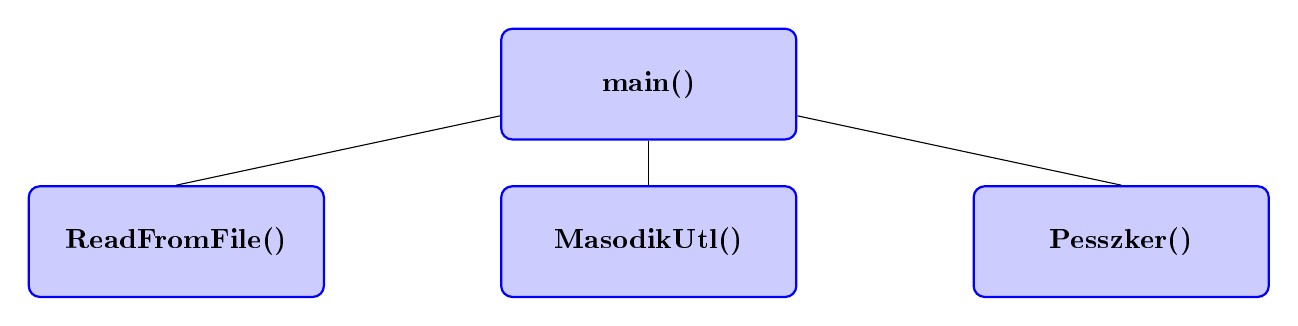
\begin{tikzpicture}
			[level distance=20mm, sibling distance=60mm, align=center, block/.style ={rectangle, draw=blue, thick, fill=blue!20,text width=10em,align=center, rounded corners, minimum height=4em}];
			\node [block] (main) {\textbf{main()}}
				[child anchor=north]
				child {node [block] (readfromfile) {\textbf{ReadFromFile()}}}
				child {node [block] (masodikutl) {\textbf{MasodikUtl()}}}
				child {node [block] (pesszker) {\textbf{Pesszker()}}};
		\end{tikzpicture}\vspace{2mm}\\
		\end{center}
	
	%% Tesztelés fejezet %%
	\fejezet{Tesztelési terv}\\
		% Fekete doboz esetek %
		\renewcommand{\labelenumi}{\Alph{enumi}.}
		\renewcommand{\labelenumii}{\arabic{enumii}.}
		{\large A feladat specifikációjára épülő (fekete doboz) tesztesetek} \vspace{2mm}\\
		Érvényes tesztesetek (most érvénytelen bemenet nem lehet):
		\begin{enumerate}		
			\item \textbf{Maximum keresés} tesztesetei:\\
			\textbf{intervallum hossza} szerint
			\begin{enumerate}
				\item \textit{nulla} hosszú: 
				\begin{itemize}[label={}]
					\item Egyetlen érték sincs (üres vagy csak elválasztójelekből álló fájl)\\
					(t1.txt: [] - válasz hamis)\\
					(t2.txt: [    ] - válasz hamis)
				\end{itemize}
				\item \textit{egy} hosszú
				\begin{itemize}[label={}]
					\item Egyetlen érték van ami pozitív\\
					(t3.txt: [4] - válasz hamis)
				\end{itemize}
				\item \textit{kettő} hosszú
				\begin{itemize}[label={}]
					\item Két egész érték\\
					(t4.txt: [asdfasd221 adsfaf] - válasz hamis)
				\end{itemize}
				\item \textit{három} hosszú
				\begin{itemize}[label={}]
					\item Nincs megoldás\\
					(t5.txt: [1dsfas ASAD2 xyy3asd] - válasz hamis)
					\item Van megoldás, első fordul elő 2-szer egymás után\\
					(t6.txt: [1dsfas 1dsfas ASAD2] válasz: igaz, 1. index, 1dsfas értékkel)
					\item Van megoldás, első fordul elő 2-szer, nem egymás után\\
					(t7.txt: [1dsfas ASAD2 1dsfas] válasz: igaz, 1. index, 1dsfas értékkel)
					\item Van megoldás, a második fordul elő 2-szer\\
					(t8.txt: [1dsfas ASAD2 ASAD2] válasz: igaz, 2. index, ASAD2 értékkel)
				\end{itemize}
				\item \textit{több} hosszú
				\begin{itemize}[label={}]
					\item Nincs megoldás\\
					(t9.txt: [KAGGSD24D1 FAFASKJE2  KAGGSD24D1 ASFLKFAAS MNBUP7AS] - válasz hamis)
					\item Egy elem fordul elő 2-szer\\
					(t10.txt: [KAGGSD24D1 FAFASKJE2  KAGGSD24D1 ASFLKFAAS MNBUP7AS] - válasz igaz, 1. index, KAGGSD24D1 értékkel)
					\item Több elem fordul elő 2-szer\\
					(t11.txt: [KAGGSD24D1 FAFASKJE2 FAFASKJE2 ASFLKFAAS MNBUP7AS] - válasz igaz, 2. index, FAFASKJE2 értékkel)
					\item Több elem fordul elő többször\\
					(t12.txt: [KAGGSD24D1 FAFASKJE2 FAFASKJE2 KAGGSD24D1 ASFLKFAAS MNBUP7AS] - válasz igaz, 2. index, FAFASKJE2 értékkel)
				\end{itemize}
			\end{enumerate}
			\item \textbf{Pesszimista keresés} tesztesetei
				\begin{enumerate}
					\item Több  elem van de nincs megoldás\\
					(t5.txt: [1dsfas ASAD2 xyy3asd] - válasz hamis)
					\item Több elem van, van megoldás\\
					(t10.txt: [KAGGSD24D1 FAFASKJE2  KAGGSD24D1 ASFLKFAAS MNBUP7AS] - válasz igaz, 1. index, KAGGSD24D1 értékkel)
					\item Több elem van, nem az első a megoldás\\
					(t12.txt: [KAGGSD24D1 FAFASKJE2 FAFASKJE2 KAGGSD24D1 ASFLKFAAS MNBUP7AS] - válasz igaz, 2. index, FAFASKJE2 értékkel)
				\end{enumerate}
		\end{enumerate}

		% Fehér doboz esetek %
		\renewcommand{\labelenumi}{\arabic{enumi}.}
		\noindent{\large A megoldó programra épülő (fehér doboz) tesztesek} \vspace{2mm}
		\setlist[enumerate,1]{leftmargin=2cm}
		\begin{enumerate}[1, itemsep=0ex]
			\item Hibás vagy nem létező állománynév megadása.
			\item Állomány nevének megadása parancssorból
			\item Ismételt futtatás kipróbálása
			\item Olyan állomány olvasása, ahol egy sorban több érték is található egyetlen illetve több szóközzel és/vagy tabulátor jellel elválasztva (t12.txt).
			\item Olyan állomány olvasása, ahol minden érték külön sorban van. (t11.txt).
			\item Főprogram ciklusának ellenőrzése: olyan bemenő adatokkal, amelyekre a ciklus egyszer sem fut le (Pl: t1.txt), pontosan egyszer fut le (Pl: t7.txt), többször lefut és igaz logikai értékkel lép ki (Pl: t10.txt), vagy hamis logikai értékkel lép ki (Pl: t9.txt).
		\end{enumerate}
\end{document}
